%%% Template originaly created by Karol Kozioł (mail@karol-koziol.net) and modified for ShareLaTeX use

%%%------------------------------------------------------------------------------------------------%%%
%%%------------------------------------%%%     PREAMBLE     %%%------------------------------------%%%
%%%------------------------------------------------------------------------------------------------%%%

\documentclass[twoside=false,a4paper,11pt]{article}

\usepackage[T1]{fontenc}
\usepackage[utf8]{inputenc}
\usepackage{graphicx}
\usepackage{xcolor}

\usepackage{tgtermes}

\usepackage{color}
\usepackage{listings}
\lstset{ %
language=SQL,                % choose the language of the code
basicstyle=\footnotesize,       % the size of the fonts that are used for the code
numbers=left,                   % where to put the line-numbers
numberstyle=\footnotesize,      % the size of the fonts that are used for the line-numbers
stepnumber=1,                   % the step between two line-numbers. If it is 1 each line will be numbered
numbersep=5pt,                  % how far the line-numbers are from the code
backgroundcolor=\color{white},  % choose the background color. You must add \usepackage{color}
showspaces=false,               % show spaces adding particular underscores
showstringspaces=false,         % underline spaces within strings
showtabs=false,                 % show tabs within strings adding particular underscores
frame=single,           % adds a frame around the code
tabsize=2,          % sets default tabsize to 2 spaces
captionpos=b,           % sets the caption-position to bottom
breaklines=true,        % sets automatic line breaking
breakatwhitespace=false,    % sets if automatic breaks should only happen at whitespace
escapeinside={\%*}{*)}          % if you want to add a comment within your code
}

\usepackage[
pdftitle={CPSC 471 Final Report}, 
pdfauthor={Timothy Mealey, Ben Roberts, Cory Jensen, Scott Saunders, University of Calgary},
colorlinks=true,linkcolor=blue,urlcolor=blue,citecolor=blue,bookmarks=true,
bookmarksopenlevel=2]{hyperref}
\usepackage{amsmath,amssymb,amsthm,textcomp}

\usepackage{enumitem}

\usepackage{multicol}
\usepackage{tikz}
\usetikzlibrary{shapes,positioning,calc}
\colorlet{lightgray}{gray!20}

\usepackage{geometry}
\geometry{total={210mm,297mm},
left=25mm,right=25mm,%
bindingoffset=0mm, top=20mm,bottom=20mm}

\linespread{1.3}

\newcommand{\linia}{\rule{\linewidth}{0.5pt}}

% custom theorems if needed
\newtheoremstyle{mytheor}
	{1ex}{1ex}{\normalfont}{0pt}{\scshape}{.}{1ex}
	{{\thmname{#1 }}{\thmnumber{#2}}{\thmnote{ (#3)}}}

\theoremstyle{mytheor}
\newtheorem{defi}{Definition}

% my own titles
\makeatletter
\renewcommand{\maketitle}{
\begin{center}
\vspace{2ex}
{\huge \textsc{\@title}}
\vspace{1ex}
\\
\linia\\
\@author \hfill \@date
\vspace{4ex}
\end{center}
}
\makeatother
%%%

% custom footers and headers
\usepackage{fancyhdr,lastpage}
\pagestyle{fancy}
\lhead{}
\chead{}
\rhead{}
\lfoot{Final Report}
\cfoot{}
\rfoot{Page \thepage\ /\ \pageref*{LastPage}}
\renewcommand{\headrulewidth}{0pt}
\renewcommand{\footrulewidth}{0pt}
%


%%%------------------------------------------------------------------------------------------------%%%
%%%------------------------------------%%%     DOCUMENT     %%%------------------------------------%%%
%%%------------------------------------------------------------------------------------------------%%%

\newcommand{\tuple}[2]{\{ #1 | #2 \}}
\newcommand{\domain}[2]{\{ (#1) | #2 \}}

\newcommand{\quantifier}[2]{(\ensuremath{#1}#2)}
\newcommand{\one}[1]{\quantifier{\exists}{#1}}
\newcommand{\all}[1]{\quantifier{\forall}{#1}}

\begin{document}

\title{CPSC 471 Final Report}
\author{Timothy Mealey, Ben Roberts, Cory Jensen, Scott Saunders}
\date{\today}
\maketitle

\section*{Abstract}

The existing tools for planning semester schedules are decentralized, making them difficult to use together. The goal with this project was to simplify the semester planning process by creating a single tool that encompassed the functionality of the UofC calendar, myUofC course search, degree navigator, and the UofC schedule builder. While we managed to implement most of the desired functionality, we did not implement the degree navigator.

\section*{Introduction}

\subsection*{Problem}

The existing tools for planning semester schedules are decentralized, making them difficult to use together. When building schedules with these tools, it is common to have more than four tabs open in one's internet browser, which is an unnecessarily complicated state for such a simple task. The goal with this project was to simplify the semester planning process by creating a single tool that encompassed the functionality of the UofC calendar, myUofC course search, degree navigator, and the UofC schedule builder.

\subsection*{Implementation}

A course search feature was built which displays course names, descriptions, prerequisites, and whether they are offered in any upcoming or current semesters. It is easily navigable using a searchable sidebar tree organized by faculty, department, and course number - selecting any of which loads that node in the main page. Selecting a node also updates the browser URL to a shareable link, without reloading the page, so that students can easily share their course planning with each other.

Similar to the courses page, the schedule page contains a sidebar tree from which one can choose courses. Differing from the courses page, this sidebar is organized by semester, using a dropdown menu, before dissecting into the different course branches. When one selects a course from the tree, its lectures, tutorials, and labs are added to a sidebar on the right. These sections can then be added to the calendar, located in the centre of the page, from this right side bar. After adding the desired sections to the calendar, the user can save their progress as a schedule.

A login system was started, from which users can be added to the database using an email and password. If a user exists in the database, they can log in using their unique credentials.

\section*{Design}

\subsection*{Users}

``Discuss the different users of your system. Your discussion in this section should be considerably more detailed than what you described for the presentation - this section should describe a complete transaction collection and, consequently, provide a complete picture of the functionality offered by your system.''

\begin{enumerate}
	\item Course Browsing
	A user interested in courses offered by the University of Calgary can navigate to the Dauwtrappen website. Once on the website, a series of SQL queries are executed which load the entire course list. These queries are executed in alphabetical order by department so that the user can begin interacting with the system before all of the data is loaded.
	Once some or all of the course data is loaded, the user can either browse through the courses using the course tree or perform a search for preferred courses by department, course numbers, and course names. Courses that fulfill their selection/search criteria display the corresponding course information such as their name and number, description, prerequisites, and when/whether they are offered.

	A user would use the Dauwtrappen website as opposed to the UofC Calender website for 3 reasons, some of which have already been mentioned:
	Firstly, the intuitive search tool.
	Secondly, the UofC Calender only mentions if courses are offered in even/odd years, but does not state which semester the courses will actually be offered in, whereas the Dauwtrappen course list does just that.
	Thirdly, the overall integration of all aspects of the Dauwtrappen website.

	\item Schedule Building
	A student or perspective student can navigate to the schedule building page of the website in order to get organized for the upcoming semester. Again, a series of SQL queries are executing which loads the course data in a cascading fashion. The user can browse through the list or use the same search tool that is present in the course selection. 
	The user can then click on a course to add it to the selected courses panel on the right side of the screen. This panel will then display the various lectures, tutorials, and labs available for that course, as well as their corresponding times. The user can individually click on these sections to add them to their schedule. To remove a selected course, the user can click the little X button on the course. This will remove it from the selected course panel and any selected sections will be removed from the schedule itself. 
	Once the user completes their schedule, they can click the save button to save their schedule to the database. They can give it a name if they wish, but this is not required.
	They may also load schedules from the database by pressing the load button and selecting the schedule they wish to load.  

	Currently the user login system is not session based, so all schedules are accessible by all users of the system.

	\item Login System

	A user who wishes to login to the website navigates to the login page. Once there, if they already have an account, they can enter their username (email) and their password, then press to login button. This executes an SQL query to confirm that have an account and that they entered the correct password. If they do not have an account, they can enter their email and a password and press the create account button. This will create an entry in the database table for that user, and they will now be able to login to the system.

	The website does not currently have sessions, so logging in does not carry over to the courses or schedule page. 

\end{enumerate}

\subsubsection*{Log In}
\subsubsection*{Course Search}
\subsubsection*{Schedule Creator}

\subsection*{Entity Relationship Diagram}

\includegraphics[width=\textwidth]{ERDiagram.png}

The red numbers on the diagram mark the changes from the initially presented diagram, and correspond to the list below.

\begin{enumerate}
	\item A prerequisite relation from Course to Course was added.
	\item Removed the ``Course Requirements'' attribute from Degree because it was redundant. It's function is handled by the Requires relation from Degree to Course.
	\item Added the ``Full Name'' attribute to Department because departments have a short code-name as well as a full English name. For example, ``CPSC'' and ``Computer Science.''
	\item A Semester entity type was added, and the Has relation from Semester to Section.
\end{enumerate}

\section*{Implementation}

\subsection*{Relational Schema Diagram}

Below you will find the relational schema diagram, which was created using the algorithm described in class that converts ERDs to RSDs. As you can see, there is a tuple for each entity type and relationship from the ER diagram, with arrows pointing from foreign keys to the primary keys they reference.

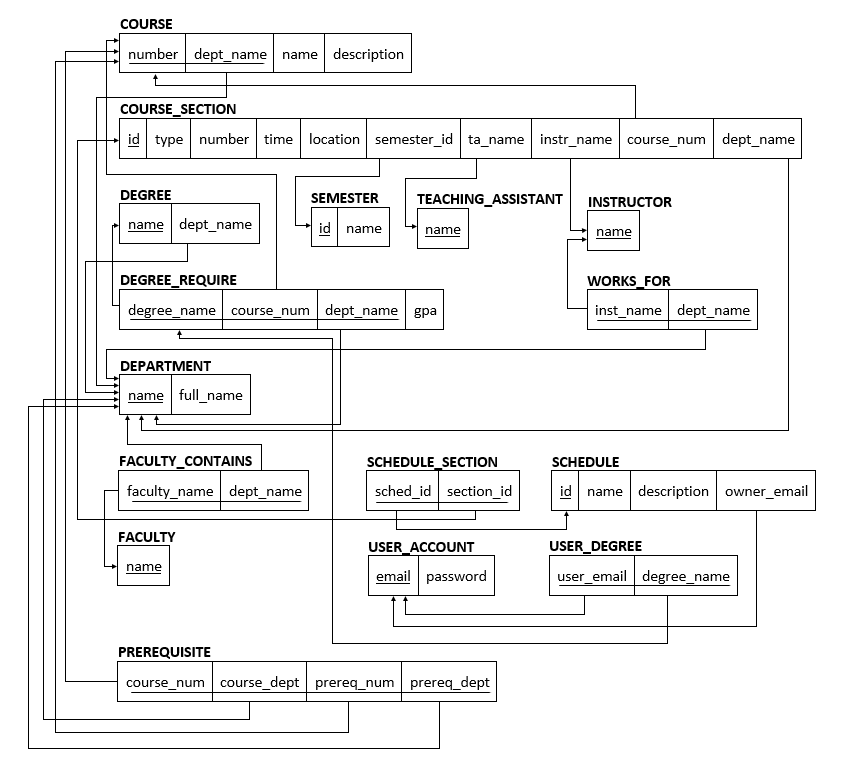
\includegraphics[width=\textwidth]{RelationalSchemaDiagram.png}

During the conversion from the ERD to the RSD, redundancies were found and required information was missing. There were also some interesting constraints put on us by the DBMS that was used. For example, the ``User'' entity was renamed to ``user\_account'' because ``user'' was a reserved keyword.

\subsection*{Database Management System}

PostgreSQL is the DBMS used because it is a full-featured SQL implementation with good support and documentation. Here are the SQL queries that were written:

Get a list of all the semesters and the faculties they contain:
\begin{lstlisting}
SELECT s.*, f.name AS fac_name
FROM faculty AS f,
	faculty_contains AS fc,
	course_section AS c,
	semester AS s
WHERE c.semester_id=s.id AND
	c.dept_name=fc.dept_name AND
	f.name=fc.faculty_name
GROUP BY s.id, f.name
\end{lstlisting}

Gets a list of all the semesters:
\begin{lstlisting}
SELECT s.* FROM semester AS s
\end{lstlisting}

Gets a list of all the course sections from a faculty in a semester:
\begin{lstlisting}
SELECT DISTINCT s.*, c.*,
	fc.faculty_name AS fac_name,
	d.full_name AS dept_full_name
FROM course AS c,
	faculty_contains AS fc,
	course_section AS s,
	department AS d
WHERE s.semester_id=<SEMESTER_ID> AND
	s.dept_name=fc.dept_name AND
	c.number=s.course_num AND
	c.dept_name=s.dept_name AND
	fc.faculty_name=<FACULTY_NAME> AND
	d.name=s.dept_name
\end{lstlisting}

Gets a list of all the course sections from a faculty:
\begin{lstlisting}
SELECT DISTINCT s.*, c.*,
	fc.faculty_name AS fac_name,
	d.full_name AS dept_full_name
FROM course AS c,
	faculty_contains AS fc,
	course_section AS s,
	department AS d
WHERE s.dept_name=fc.dept_name AND
	c.number=s.course_num AND
	c.dept_name=s.dept_name AND
	fc.faculty_name=<FACULTY_NAME> AND
	d.name=s.dept_name
\end{lstlisting}

Checks if a user exists in the database with a given email and password:
\begin{lstlisting}
SELECT email, password
FROM user_account
WHERE email=<EMAIL> AND password=<PASSWORD>
\end{lstlisting}

Checks if a user exists in the database with a given email:
\begin{lstlisting}
SELECT email
FROM user_account
WHERE email=<EMAIL>
\end{lstlisting}

Adds a user account to the database with an email and password:
\begin{lstlisting}
INSERT INTO user_account
VALUES (<EMAIL>, <PASSWORD>)
\end{lstlisting}

There are many more INSERT queries in the various scrapers and test-data scripts that populate the database with course information. These have been left out to shorten this document.

\subsection*{User Interface}

``Present a brief description of your interface design, including several screenshots.''

\end{document}
